\documentclass{article}
% Language setting
% Replace `english' with e.g. `spanish' to change the document language
\usepackage{biblatex} %Imports biblatex package
\addbibresource{sample.bib}
\usepackage{changepage}
\usepackage[english]{babel}
\usepackage{tikz}
\usepackage{array}
\usepackage{amsmath}
\usepackage{accents}
\usepackage{empheq}
\usepackage{pythonhighlight}
\newcolumntype{P}[1]{>{\centering\arraybackslash}p{#1}}
\newcolumntype{M}[1]{>{\centering\arraybackslash}m{#1}}

% Set page size and margins
% Replace `letterpaper' with `a4paper' for UK/EU standard size
\usepackage[letterpaper,top=2cm,bottom=2cm,left=3cm,right=3cm,marginparwidth=1.75cm]{geometry}

\usepackage{graphicx}
\usepackage[colorlinks=true, allcolors=blue]{hyperref}
\usepackage{setspace}
\usepackage{booktabs}
\usepackage[T1]{fontenc}
\usepackage{longtable}
\doublespacing

\begin{document}
\newcommand{\circled}[1]{\tikz[baseline=(char.base)]{
            \node[shape=circle,draw,inner sep=2pt] (char) {#1};}}

\newcommand{\pd}[3]{\frac{\partial^{#3}#1}{\partial {#2}^{#3}}}
\begin{titlepage}

\centering
\scshape
\vspace{\baselineskip}

%
\rule{\textwidth}{1.6pt}\vspace*{-\baselineskip}\vspace*{2pt}
\rule{\textwidth}{0.4pt}

{\Huge \textbf{\textsc{NPRE 449: Homework 7 \\
\vspace{15pt}}}}

\rule{\textwidth}{0.4pt}\vspace*{-\baselineskip}\vspace{3.2pt}
\rule{\textwidth}{1.6pt}\vspace{6pt}
%%\centerline{\textit{University of Illinois at Urbana-Champaign}} 
\vspace{1.5\baselineskip}


\large \centerline{\textbf{Author:} Nathan Glaser}
\large \centerline{\textbf{Net-ID:} nglaser3}
\quad

\vfill
\large \centerline{September 18, 2024}
%
\pagenumbering{gobble}
\end{titlepage}

\tableofcontents
\newpage
\pagenumbering{arabic}

\section{Question 1}
To begin, our differential equations for single phase, 1-D are:

\begin{subequations}
    \begin{equation}
        \pd{\rho}{t}{} + \pd{\rho v}{z}{} = 0
        \label{mass}
    \end{equation}
    \begin{equation}
        \pd{\rho v}{t}{} + \pd{}{z}{}\rho v^2 = -\pd{P}{z}{}-\tau_F\frac{\xi_w}{A_f} - \rho g \sin(\theta)
        \label{momentum}
    \end{equation}
    \begin{equation}
        \pd{\rho h}{t}{} + \pd{}{z}{}\rho v h = \frac{q''\xi_h}{A}+\pd{P}{t}{} + q'''
        \label{energy}
    \end{equation}
\end{subequations}

Now, we apply our simplifications. Assuming steady state, substituting in $G = \rho v$, the pipe is horizontal (i.e. $\theta = 0$), $h = c_pT$, incompressible, and no heat-generation:

\begin{subequations}
    \begin{equation}
        \pd{G}{z}{} = 0
        \label{ssmass}
    \end{equation}
    \begin{equation}
        \pd{}{z}{}\frac{G^2}{\rho} = -\pd{P}{z}{} - \tau_F\frac{\xi_w}{A_f}
        \label{ssmomentum}
    \end{equation}
    \begin{equation}
         c_p\pd{GT}{z}{} = \frac{q''\xi_h}{A}
    \end{equation}
\end{subequations}

From the mass equation, \eqref{ssmass}, we see the mass flux is constant. Further, the definition of $\tau_F$ is $\frac{fG^2}{2\rho}$. Thus, the momentum and energy equations simplify further:
\begin{subequations}
    \begin{equation}
        -\pd{P}{z}{} = \frac{fG^2\xi_w}{2\rho A_f}
    \end{equation}
    \begin{equation}
        c_pG\pd{T}{z}{} = \frac{q''\xi_h}{A}
    \end{equation}
\end{subequations}

Now, solving our energy equation we can find the temperature distribution:

\begin{subequations}
    \begin{equation}
        \pd{T}{z}{}=\frac{q''\xi_h}{c_pGA}
    \end{equation}
    \begin{equation}
        \int_0^l\partial T  = \int_0^l\frac{q''\xi_h}{c_pGA}\partial z
    \end{equation}
    \begin{equation}
        T(l) - T(0) = \frac{q''\xi_h}{c_pGA} l
    \end{equation}
    \begin{equation}
        \frac{\Delta Tc_pGA}{q''\xi_h} = l
    \end{equation}
    \begin{equation}
        \boxed{l = 6.652\ m}
    \end{equation}
\end{subequations}

where material properties were evaluated at the average temperature of the fluid, $50/ ^oC$.

To find the surface temperature at the exit, we utilize newtons law of cooling:

\begin{equation}
    q'' = h(T_s(z) - \Bar{T}(z))
    \label{newtons}
\end{equation}

To find h, we must first determine which correlation to use. Thus we find the Reynolds number, $\frac{GD}{\mu}$, as 598.85 (using material properties at $80\ ^oC$. Thus the flow is laminar and because it is fully developed in a pipe, we can use $Nu = 4.36$. Thus, using the definition for $Nu= \frac{hD}{k}$, we can solve for h. Using material properties of water at Standard pressure and $80\ ^oC$, we find h to be 48.468. Thus, plugging in all known values into Eq. \ref{newtons}, and solving for $T_s$:

\begin{subequations}
    \begin{equation}
        T_s(l) = \frac{q''}{h} + \Bar{T}(l)
    \end{equation}
    \begin{equation}
        \boxed{T_s(l) = 121.264}
    \end{equation}
\end{subequations}

\newpage
\section{Question 2}

To begin, our governing equations for the fluid, assuming steady state, are:

\begin{subequations}
    \begin{equation}
        \pd{G}{z}{} = 0
    \end{equation}
    \begin{equation}
        G^2\pd{}{z}{}\frac{1}{\rho} = -\pd{P}{z}{} - \tau_F\frac{\xi_w}{A_f} - \rho g \sin(\theta)
    \end{equation}
    \begin{equation}
        c_pG\pd{T_f}{z}{} = \frac{q''\xi_h}{A}+q'''
    \end{equation}
\end{subequations}

Assuming incompressibility, horizontal pipe, and no heat generation in our fluid the momentum and energy equations simplify to:

\begin{subequations}
    \begin{equation}
        -\pd{P}{z}{} = \tau_F\frac{\xi_w}{A_f} = \frac{fG^2\xi_w}{2\rho A_f}
    \end{equation}
    \begin{equation}
        c_pG\pd{T_f}{z}{} = \frac{q''\xi_h}{A}
    \end{equation}
\end{subequations}

Then, through control volume analysis, we can relate $q'''$ in the wall to the heat flux into the fluid:

\begin{equation}
    q''A_s = q'''V_p
\end{equation}

 plugging this back into the energy equation and solving for the temperature distribution:

 \begin{subequations}
     \begin{equation}
         \pd{T_f}{z}{} = \frac{q'''V_p\xi_h}{c_pGA_fA_s}
     \end{equation}
     \begin{equation}
         T_f(z) = \frac{q'''V_p\xi_h}{c_pGA_fA_s} z + T_0
     \end{equation}
     \begin{equation}
         T_f(z) = \frac{q'''\pi h(r^2_o - r^2_i)(2\pi r_i)}{c_pG(\pi r_i^2)(2\pi r_ih)}z + T_0
     \end{equation}
 \end{subequations}

plugging in l for z, we can solve for l:
\begin{subequations}
    \begin{equation}
        T_f(z) = \frac{q'''(r^2_o - r^2_i)}{c_pG(\ r_i^2)}z + T_0
    \end{equation}
    \begin{equation}
       l = \frac{\Delta Tc_pG( r_i^2)}{q'''(r^2_o - r^2_i)}
    \end{equation}
    \begin{equation}
        \boxed{l = 17.734\ m}
    \end{equation}
\end{subequations}

Next to solve for the heat transfer coefficient we simply solve newtons law of cooling for h:

\begin{subequations}
    \begin{equation}
        q'' = h(T_s - \Bar{T})
    \end{equation}
    \begin{equation}
        h = \frac{q''}{T_s - \Bar{T}}
    \end{equation}
    \begin{equation}
        \boxed{h = 1500}
    \end{equation}
\end{subequations}

Next, to solve for the heat transfer coefficient we first solve for the Reynolds: $Re = \frac{GD}{\mu} = 9749.467$. Thus our flow is turbulent, and we will use the Dittus-Boelter correlation to find h:
\begin{equation}
    Nu = 0.023Re^{0.8}Pr^{0.3}
\end{equation}

Thus our Nusselt number is 55.485, and then solving for h we get:

\begin{equation}
    \boxed{h = 2114.197}
\end{equation}

\section{Question 3}

First, performing an energy balance, we can determine how much heat was lost by the hot air. 

\begin{equation}
    \Dot{E}_{loss} = \Dot{m}c_p\Delta T 
\end{equation}

\begin{equation}
    \boxed{\Dot{E}_{loss} = 1300.65 W}
\end{equation}
Further, we can relate the heat loss by the air to the heat flux due to convection by:

\begin{equation}
    hA_s\Delta T_{air,o} = q''A_s= \Dot{m}c_p\Delta T_{air,i}
\end{equation}

thus q'' is simply:

\begin{equation}
    \boxed{q'' = \frac{\Dot{m}c_p\Delta T_{air,i}}{A_s} = 552.013}
\end{equation}

and then, because the ambient air is at $o^C$, the $\Delta T_{air,o}$ is simply the surface temperature of the duct:
\begin{equation}
    \boxed{T_s = \frac{q''}{h} = 92.002}
\end{equation}

\section{Question 4}

To begin, the governing equations for this fluid are:

\begin{subequations}
    \begin{equation}
        \label{mass}
        \pd{G}{z}{} = 0
    \end{equation}
    \begin{equation}
        \label{momentum}
        G^2\pd{}{z}{}\frac{1}{\rho} = -\pd{P}{z}{} - \tau_F\frac{\xi_w}{A_f}
    \end{equation}
    \begin{equation}
        \label{energy}
        c_pG\pd{T_f}{z}{} = \frac{q''\xi_h}{A}
    \end{equation}
\end{subequations}

However, for this problem set-up we only care about the energy equation. Thus, solving this equation:
\newcommand{\const}{\frac{h \xi_h}{c_pAG}}
\begin{subequations}
    \begin{equation}
        \pd{T_f}{z}{} = \frac{q''\xi_h}{c_pAG}
    \end{equation}
    \begin{equation}
        \pd{\theta}{z}{} = \const \theta (z)
    \end{equation}
    \begin{equation}
        \theta(z) = \theta_0 e^{\const z}
    \end{equation}
    \begin{equation}
        T_f(z) = T_{s} - \left( T_s - T_{f,in} \right) e^{-\const z}
    \end{equation}
\end{subequations}

To find h, we first determine reynolds number. We find Re to be $397.888$, and thus it is a laminar pipe. Hence, we use a constant Nusselt number: $3.66$. Finally, we find h to simply be: $10.102$. Plugging this in, and solving for $T_f(L)$, we find the outlet temperature to be:

\begin{equation}
    \boxed{T_f(L) = 24.751 ^oC}
\end{equation}

Next, to find the heat transfer rate we utilize $\Dot{m}c_p \Delta T$:
\begin{subequations}
    \begin{equation}
        q = \Dot{m}c_p \Delta T
    \end{equation}
    \begin{equation}
        \boxed{q = 5062.139\ W}
    \end{equation}
\end{subequations}


\section{Question 5}

To begin, the governing equations for this fluid are:

\begin{subequations}
    \begin{equation}
        \label{mass}
        \pd{G}{z}{} = 0
    \end{equation}
    \begin{equation}
        \label{momentum}
        G^2\pd{}{z}{}\frac{1}{\rho} = -\pd{P}{z}{} - \tau_F\frac{\xi_w}{A_f}
    \end{equation}
    \begin{equation}
        \label{energy}
        c_pG\pd{T_f}{z}{} = \frac{q''\xi_h}{A}
    \end{equation}
\end{subequations}

Solving the energy equation:
\begin{subequations}
    \begin{equation}
        \pd{T_f}{z}{} = \frac{q''\xi_h}{c_pAG}
    \end{equation}
    \begin{equation}
        \pd{\theta}{z}{} = \const \theta (z)
    \end{equation}
    \begin{equation}
        \theta(z) = \theta_0 e^{\const z}
    \end{equation}
    \begin{equation}
        T_f(z) = T_{s} - \left( T_s - T_{f,in} \right) e^{-\const z}
    \end{equation}
\end{subequations}

Solving this equation for L, the distance required to heat the pipe to 75 $^o C$:

\begin{subequations}
    \begin{equation}
        T_f(z) = T_{s} - \left( T_s - T_{f,in} \right) e^{-\const z}
    \end{equation}
    \begin{equation}
        \frac{\theta (z)}{\theta_0} = e^{-\const L}
    \end{equation}
    \begin{equation}
        \ln\left( \frac{\theta (z)}{\theta_0} \right) = \const L
    \end{equation}
    \begin{equation}
        L = \ln\left( \frac{\theta (z)}{\theta_0} \right) 
        \left[ \frac{c_pAG}{h\xi_h} \right]
    \end{equation}
    \begin{equation}
        h = \frac{Nuk}{D} = \frac{0.023 (\frac{GD}{\mu})^{0.8} (\frac{\mu c_p}{k})^{0.4}k}{D} = 6918.149
    \end{equation}
    \begin{equation}
        \boxed{L = 10.563 m}
    \end{equation}
\end{subequations}

Next, to find the pressure drop, we investigate the momentum equation:
\begin{subequations}
    \begin{equation}
        -\pd{P}{z}{} = \tau_f \frac{\xi_w}{A_f}
    \end{equation}
    \begin{equation}
        \Delta P = \frac{fG^2\xi_w l}{2\rho A_f}
    \end{equation}
\end{subequations}

where $f$ is found via investigation of the Reynolds number. Recalling the Reynolds number as $116415.220$. 

\begin{equation}
    f = (0.79 \ln{Re} - 1.64)^{-2} = \boxed{0.0174}
\end{equation}

Then:

\begin{subequations}
    \begin{equation}
        \Delta P = \frac{fG^2\xi_w L}{2\rho A_f}
    \end{equation}
    \begin{equation}
        \Delta P = \frac{f \rho u^2  (\pi D) L}{2 (\pi /4 D^2)}
    \end{equation}
    \begin{equation}
        \Delta P = \frac{2 f \rho u^2 L}{D}
    \end{equation}
    \begin{equation*}
        Substituting\ in\ \frac{f}{4}\ for\ f:
    \end{equation*}
    \begin{equation}
        \Delta P = \frac{f G^2 L }{2\rho D}
    \end{equation}
    \begin{equation}
        \boxed{\Delta P = 5899.008\ kPa}
    \end{equation}
\end{subequations}



Then, to solve for the pipe length and pressure drop as a function of $\Dot{m}$ and D:

\begin{figure}
    \centering
    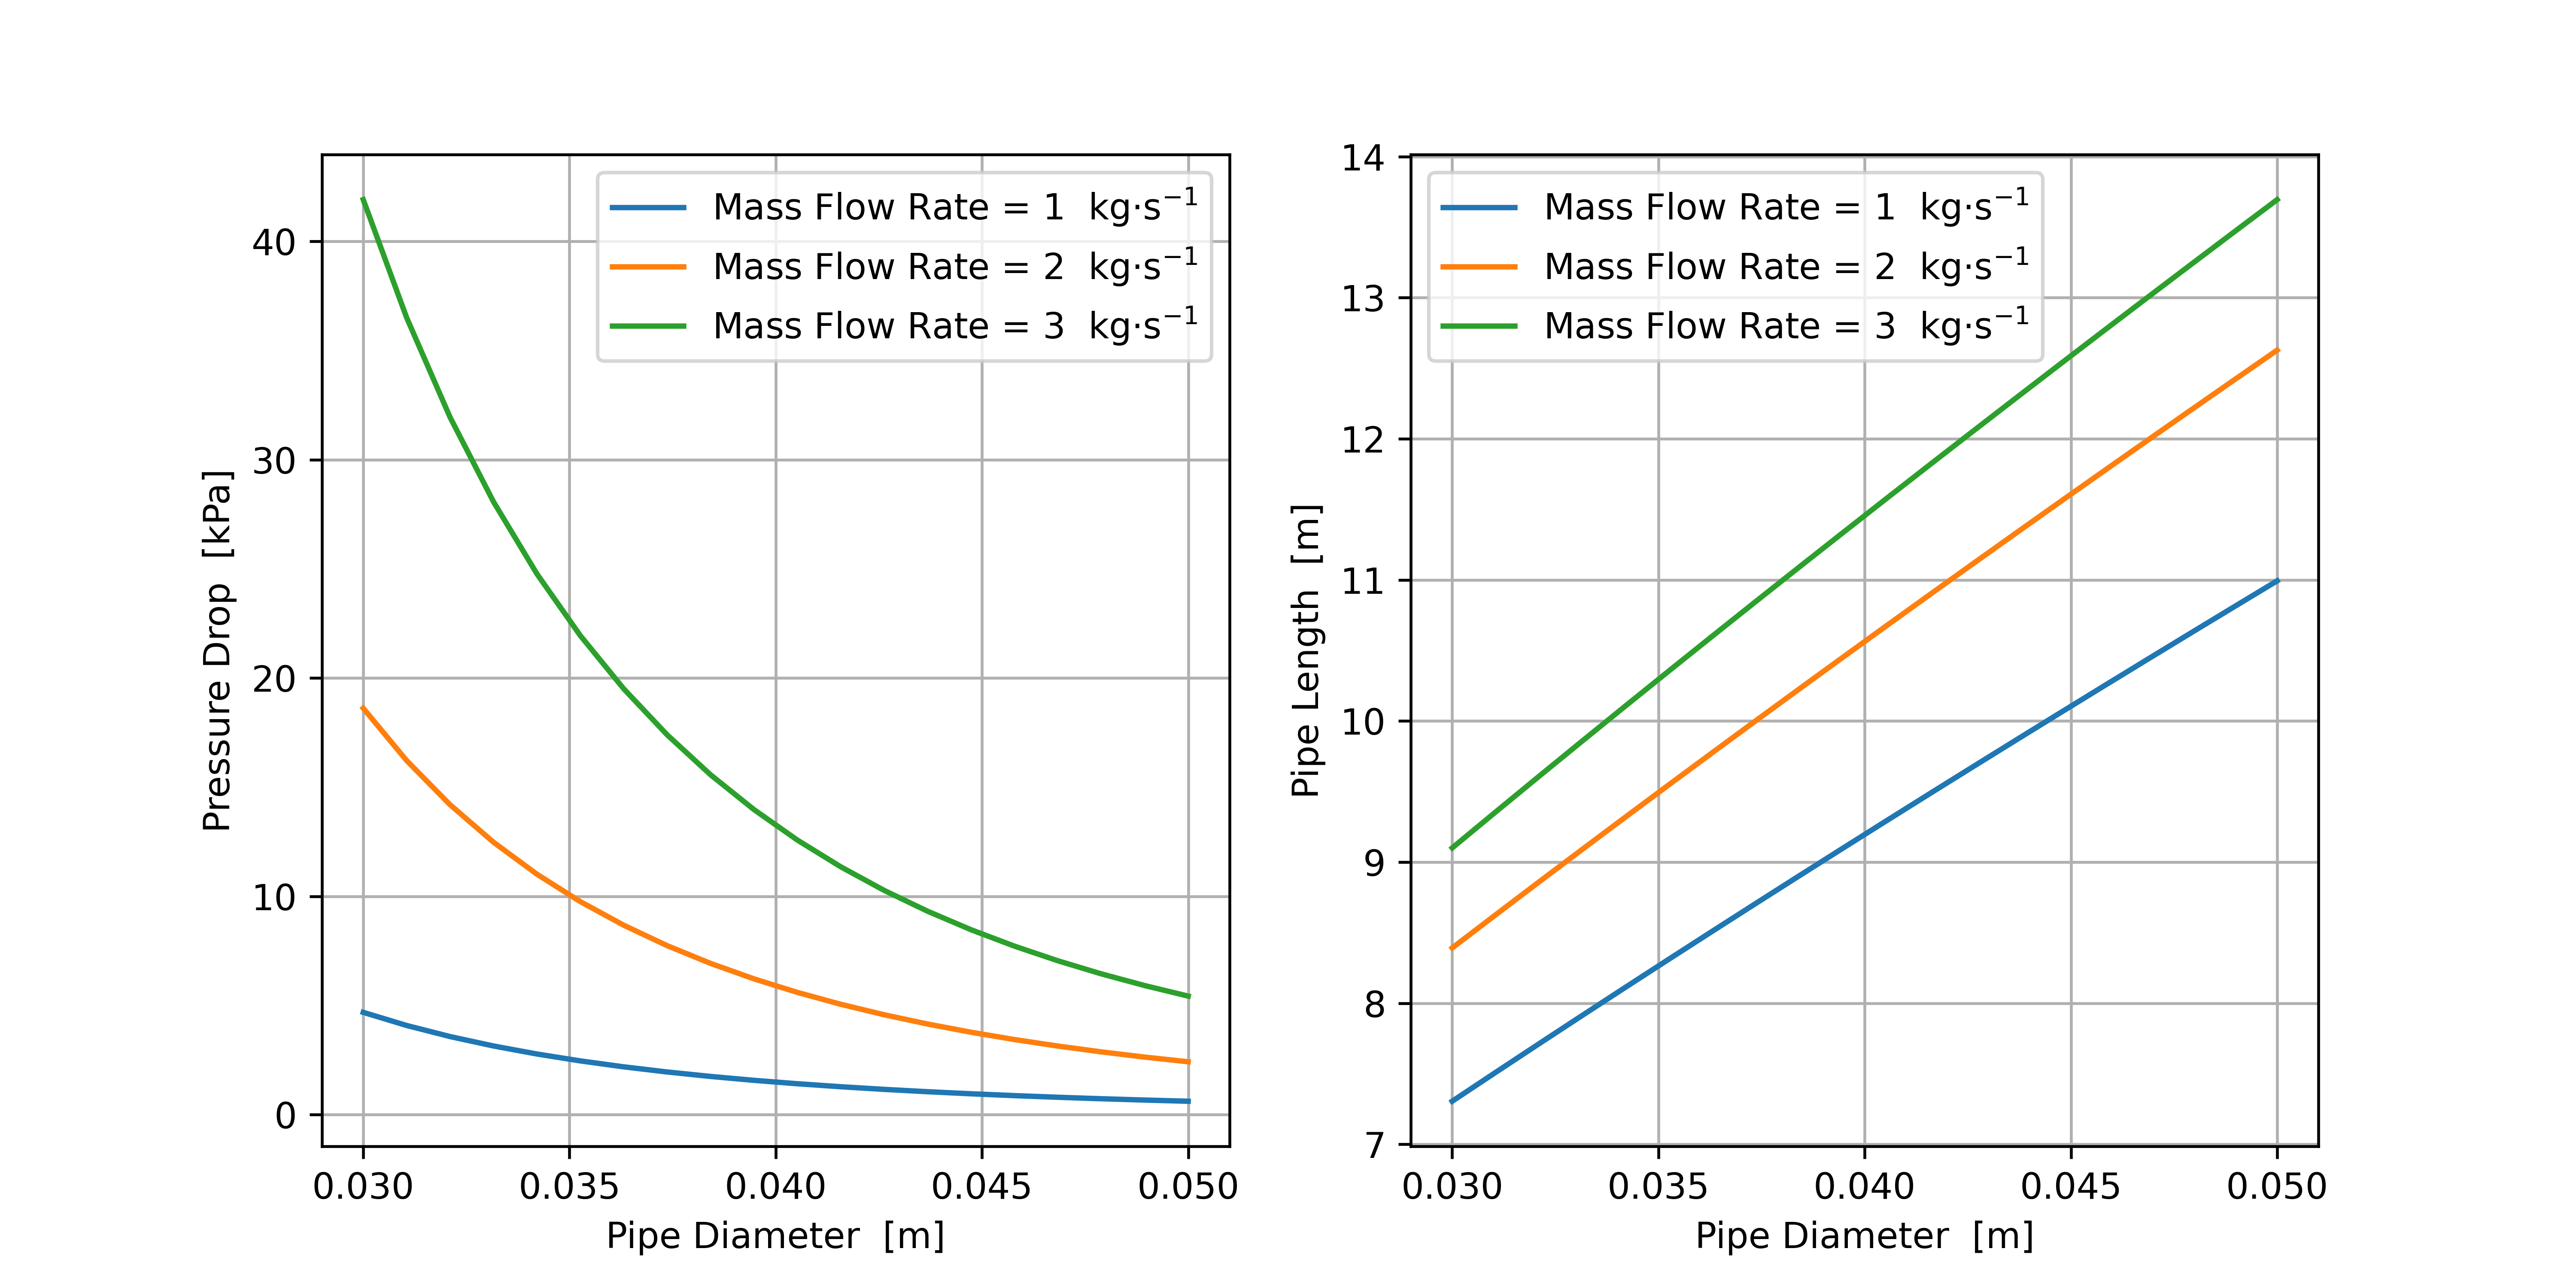
\includegraphics[width=\linewidth]{simple.png}
    \caption{Pressure Drop (left) and Pipe Length (right)}
    \label{fig:enter-label}
\end{figure}

Or in much prettier form:

\begin{figure}[!hp!]
    \centering
    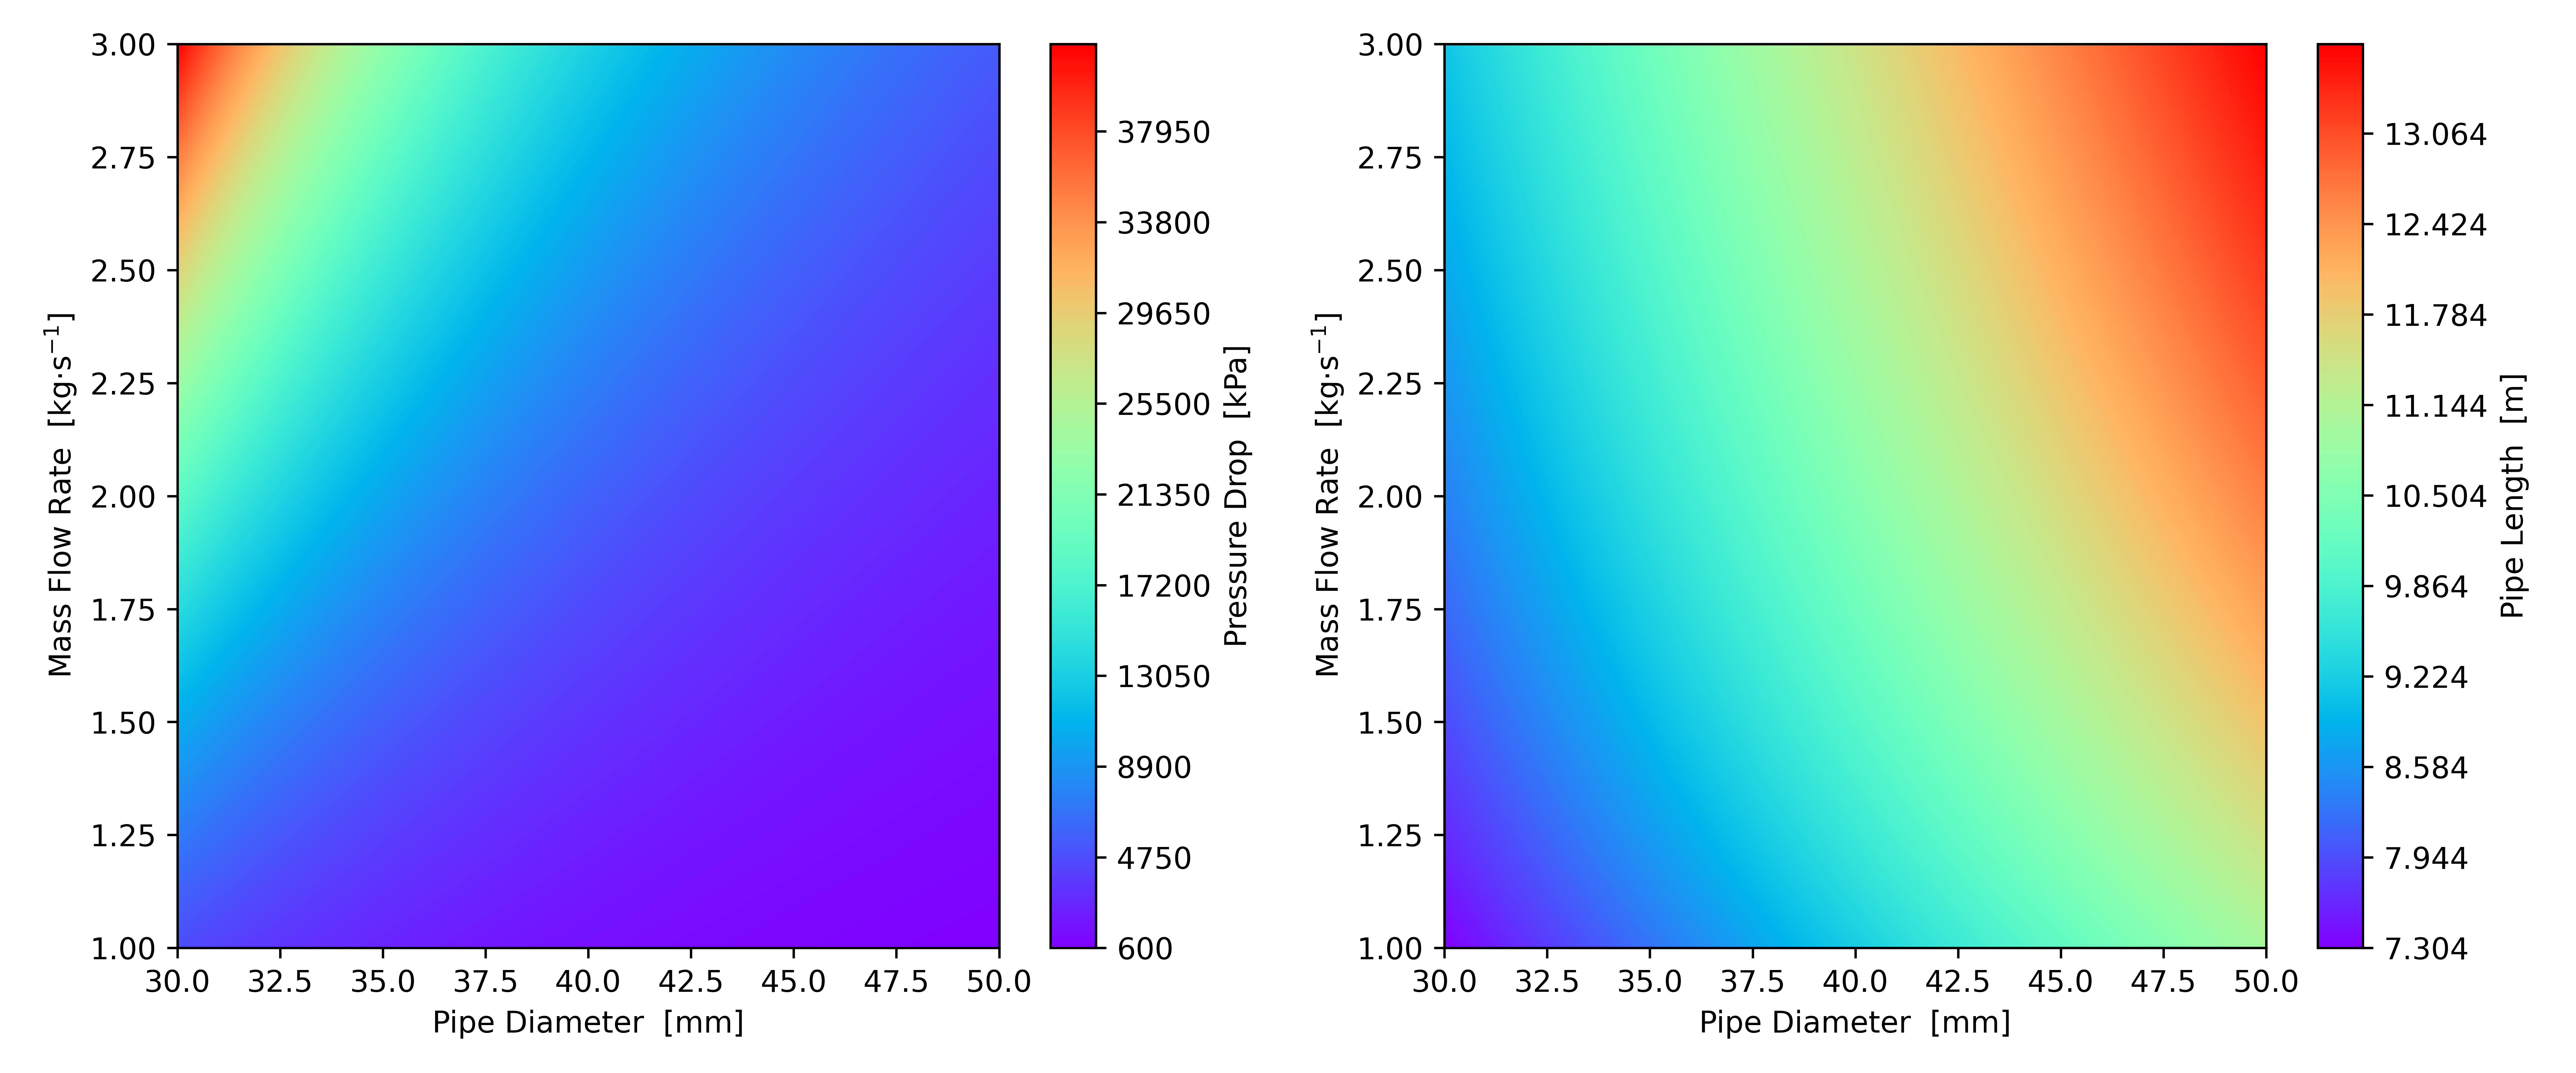
\includegraphics[width=\linewidth]{contour.png}
    \caption{Pressure Drop (left) and Pipe Length (right)}
    \label{fig:pipelength}
\end{figure}

\section{Question 6}
find expression relating q'',q', and q'''. 

Find $T_f$ as a function of z
\end{document}